% ==========================================================================
%  Edney type IV interaction, close-up with jet shock-cell structure
%
%  Standalone LaTeX document.  On Overleaf: New Project > Blank Project,
%  replace ALL of main.tex with this file (or upload it and set it as the
%  main document) and compile with pdfLaTeX.  In the paper, include the
%  compiled PDF with \includegraphics.
%
%  Generated by make_figures.py; coordinates in mm, origin at the cylinder
%  centre, x downstream, y up.
%  Case: M_inf = 8.03, beta = 18.1 deg -> theta = 12.49 deg, M_2 = 5.252 (gamma = 1.4).
%  R = 38.1 mm, inlet radius 150.39 mm, outlets at phi = +/-65 deg, no-slip wall
%  |phi| <= 45 deg, slip wall beyond, inlet split phi = -12.25 deg.
%  Jet: transmitted shock -26.2 deg -> jet direction -15.2 deg,
%  M_jet = 2.40, width 4.5 mm (oblique-shock relations).
%  Jet arch, jet bow shock stand-off and shock cells are schematic.
%  Shock cells: compressions solid, expansion fans dashed (state this in the caption).
% ==========================================================================
\documentclass[border=1pt]{standalone}
% ---- fonts: Helvetica text; sans-serif math (newtxsf) when available
\usepackage[T1]{fontenc}
\usepackage[scaled=0.92]{helvet}
\renewcommand{\familydefault}{\sfdefault}
\IfFileExists{newtxsf.sty}{\usepackage{newtxsf}}{}
\usepackage{tikz}
\usetikzlibrary{arrows.meta}

% ---- colours
\definecolor{ink}{HTML}{111111}
\definecolor{shockgrey}{HTML}{4A4A4A}
\definecolor{dimgrey}{HTML}{808080}
\definecolor{leadergrey}{HTML}{9A9A9A}
\definecolor{bodygrey}{HTML}{E4E4E4}
\definecolor{freeblue}{HTML}{1A5FA8}
\definecolor{postgreen}{HTML}{0E8A62}
\definecolor{slipochre}{HTML}{B06A10}
\definecolor{jetfill}{HTML}{FBEBD3}
\definecolor{zoomred}{HTML}{C0392B}

% ---- styles
\tikzset{
  lbl/.style={font=\sffamily\small, text=ink, inner sep=1.2pt, align=center},
  sml/.style={font=\sffamily\footnotesize, text=ink, inner sep=1.2pt, align=center},
  region/.style={font=\sffamily\small, text=dimgrey, inner sep=1pt},
  leader/.style={draw=leadergrey, line width=0.4pt},
  freeinlet/.style={draw=freeblue, line width=1.5pt},
  postinlet/.style={draw=postgreen, line width=1.5pt},
  outlet/.style={draw=dimgrey, line width=1.1pt, dash pattern=on 3.2pt off 2pt, line cap=butt},
  noslip/.style={draw=ink, line width=1.7pt},
  slip/.style={draw=slipochre, line width=1.7pt, dash pattern=on 2pt off 1.1pt, line cap=butt},
  shockA/.style={draw=shockgrey, line width=0.7pt},
  shockB/.style={draw=ink, line width=1.1pt},
  jetshock/.style={draw=ink, line width=1.1pt},
  shear/.style={draw=ink, line width=0.7pt, dash pattern=on 2.4pt off 1.4pt, line cap=butt},
  cellshock/.style={draw=ink, line width=0.45pt},
  fan/.style={draw=ink, line width=0.45pt, dash pattern=on 1.4pt off 0.9pt, line cap=butt},
  hatch/.style={draw=dimgrey, line width=0.35pt, line cap=butt},
  flow/.style={line width=0.9pt, -{Stealth[length=2.4mm, width=1.8mm]}},
  jetflow/.style={draw=ink, line width=0.75pt, -{Stealth[length=2mm, width=1.5mm]}},
  dim/.style={draw=dimgrey, line width=0.45pt,
              {Stealth[length=1.6mm, width=1.1mm]}-{Stealth[length=1.6mm, width=1.1mm]}},
  triple/.style={circle, fill=ink, inner sep=0pt, minimum size=1.6mm},
  dot/.style={circle, fill=leadergrey, inner sep=0pt, minimum size=1mm},
  panel/.style={font=\sffamily\bfseries\small, inner sep=0pt},
  % grid
  gridline/.style={draw=ink, line width=0.12pt},
  gridedge/.style={draw=ink, line width=0.6pt},
  axis/.style={draw=ink, line width=0.5pt},
  tick/.style={draw=ink, line width=0.4pt},
  ticklbl/.style={font=\sffamily\footnotesize, text=ink, inner sep=1.5pt},
  zoombox/.style={draw=zoomred, line width=0.6pt},
}
% panel letter: change to \newcommand{\panellabel}{} to remove it
\newcommand{\panellabel}{(b)}

\begin{document}
\sffamily\small
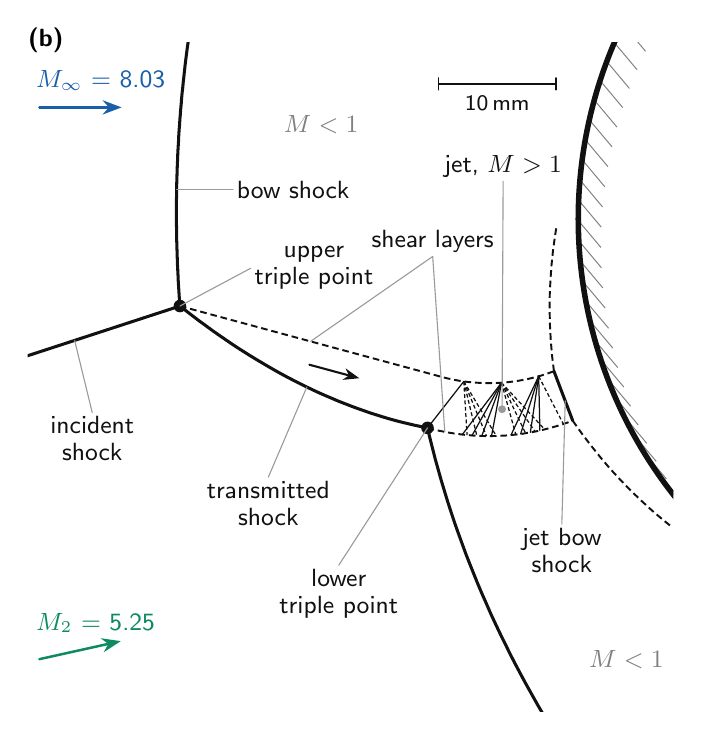
\begin{tikzpicture}[x=1mm, y=1mm, line cap=round, line join=round]

\begin{scope}[shift={(126.73,62.62)}, x=1.49091mm, y=1.49091mm]
  \begin{scope}
    \clip (-85,-42) rectangle (-30,15);
    % body and wall
    \fill[white] (0,0) circle[radius=38.1];
    \begin{scope}
      \clip (0,0) circle[radius=38.1];
      \draw[hatch] (-19.18,-32.84) -- (-17.12,-35.29);
      \draw[hatch] (-20.66,-31.94) -- (-18.6,-34.4);
      \draw[hatch] (-22.09,-30.98) -- (-20.03,-33.43);
      \draw[hatch] (-23.48,-29.95) -- (-21.42,-32.4);
      \draw[hatch] (-24.82,-28.86) -- (-22.77,-31.31);
      \draw[hatch] (-26.11,-27.71) -- (-24.06,-30.16);
      \draw[hatch] (-27.35,-26.5) -- (-25.29,-28.96);
      \draw[hatch] (-28.53,-25.24) -- (-26.47,-27.69);
      \draw[hatch] (-29.65,-23.93) -- (-27.6,-26.38);
      \draw[hatch] (-30.72,-22.56) -- (-28.66,-25.01);
      \draw[hatch] (-31.71,-21.15) -- (-29.66,-23.6);
      \draw[hatch] (-32.65,-19.7) -- (-30.59,-22.15);
      \draw[hatch] (-33.52,-18.2) -- (-31.46,-20.65);
      \draw[hatch] (-34.31,-16.67) -- (-32.26,-19.12);
      \draw[hatch] (-35.04,-15.1) -- (-32.99,-17.55);
      \draw[hatch] (-35.7,-13.5) -- (-33.64,-15.95);
      \draw[hatch] (-36.28,-11.87) -- (-34.22,-14.32);
      \draw[hatch] (-36.79,-10.22) -- (-34.73,-12.67);
      \draw[hatch] (-37.22,-8.55) -- (-35.16,-11);
      \draw[hatch] (-37.58,-6.86) -- (-35.52,-9.31);
      \draw[hatch] (-37.86,-5.15) -- (-35.8,-7.6);
      \draw[hatch] (-38.06,-3.43) -- (-36,-5.88);
      \draw[hatch] (-38.18,-1.71) -- (-36.13,-4.16);
      \draw[hatch] (-38.23,0.02) -- (-36.17,-2.43);
      \draw[hatch] (-38.2,1.75) -- (-36.14,-0.7);
      \draw[hatch] (-38.08,3.47) -- (-36.03,1.02);
      \draw[hatch] (-37.89,5.19) -- (-35.84,2.74);
      \draw[hatch] (-37.63,6.9) -- (-35.57,4.45);
      \draw[hatch] (-37.28,8.59) -- (-35.22,6.14);
      \draw[hatch] (-36.86,10.27) -- (-34.8,7.82);
      \draw[hatch] (-36.36,11.93) -- (-34.31,9.48);
      \draw[hatch] (-35.79,13.56) -- (-33.74,11.11);
      \draw[hatch] (-35.15,15.16) -- (-33.09,12.71);
      \draw[hatch] (-34.43,16.74) -- (-32.37,14.28);
      \draw[hatch] (-33.64,18.27) -- (-31.59,15.82);
      \draw[hatch] (-32.79,19.78) -- (-30.73,17.32);
      \draw[hatch] (-31.86,21.24) -- (-29.81,18.79);
      \draw[hatch] (-30.87,22.66) -- (-28.82,20.2);
      \draw[hatch] (-29.82,24.03) -- (-27.76,21.58);
      \draw[hatch] (-28.71,25.35) -- (-26.65,22.9);
      \draw[hatch] (-27.54,26.62) -- (-25.48,24.17);
      \draw[hatch] (-26.31,27.84) -- (-24.25,25.38);
      \draw[hatch] (-25.02,28.99) -- (-22.97,26.54);
      \draw[hatch] (-23.69,30.09) -- (-21.63,27.64);
      \draw[hatch] (-22.31,31.13) -- (-20.25,28.68);
      \draw[hatch] (-20.88,32.11) -- (-18.82,29.66);
      \draw[hatch] (-19.41,33.01) -- (-17.35,30.56);
    \end{scope}
    \draw[noslip, line width=2pt] (135:38.1) arc[start angle=135, end angle=225, radius=38.1];
    \draw[slip, line width=2pt] (115:38.1) arc[start angle=115, end angle=135, radius=38.1];
    \draw[slip, line width=2pt] (225:38.1) arc[start angle=225, end angle=245, radius=38.1];

    % bow shock (upper and lower branches) and incident shock
    \draw[shockB]
      (-72.03,-7.42) -- (-72.06,-7.1) -- (-72.08,-6.78) -- (-72.1,-6.46) -- (-72.12,-6.14) --
      (-72.14,-5.82) -- (-72.16,-5.5) -- (-72.18,-5.18) -- (-72.19,-4.86) --
      (-72.21,-4.54) -- (-72.22,-4.22) -- (-72.24,-3.91) -- (-72.25,-3.59) --
      (-72.26,-3.27) -- (-72.27,-2.95) -- (-72.28,-2.63) -- (-72.29,-2.31) --
      (-72.3,-1.99) -- (-72.31,-1.67) -- (-72.31,-1.35) -- (-72.32,-1.03) --
      (-72.32,-0.71) -- (-72.33,-0.39) -- (-72.33,-0.07) -- (-72.33,0.25) -- (-72.33,0.56) --
      (-72.33,0.88) -- (-72.33,1.2) -- (-72.33,1.52) -- (-72.32,1.84) -- (-72.32,2.16) --
      (-72.31,2.48) -- (-72.31,2.8) -- (-72.3,3.12) -- (-72.29,3.44) -- (-72.28,3.76) --
      (-72.27,4.08) -- (-72.26,4.4) -- (-72.25,4.72) -- (-72.23,5.04) -- (-72.22,5.35) --
      (-72.21,5.67) -- (-72.19,5.99) -- (-72.17,6.31) -- (-72.15,6.63) -- (-72.14,6.95) --
      (-72.12,7.27) -- (-72.1,7.59) -- (-72.07,7.91) -- (-72.05,8.23) -- (-72.03,8.55) --
      (-72,8.87) -- (-71.98,9.19) -- (-71.95,9.51) -- (-71.92,9.82) -- (-71.9,10.14) --
      (-71.87,10.46) -- (-71.84,10.78) -- (-71.8,11.1) -- (-71.77,11.42) -- (-71.74,11.74) --
      (-71.7,12.06) -- (-71.67,12.38) -- (-71.63,12.7) -- (-71.6,13.02) -- (-71.56,13.34) --
      (-71.52,13.66) -- (-71.48,13.98) -- (-71.44,14.29) -- (-71.4,14.61) --
      (-71.35,14.93) -- (-71.31,15.25) -- (-71.27,15.57) -- (-71.22,15.89) --
      (-71.17,16.21) -- (-71.13,16.53) -- (-71.08,16.85) -- (-71.03,17.17) --
      (-70.98,17.49) -- (-70.93,17.81) -- (-70.87,18.13) -- (-70.82,18.45) --
      (-70.77,18.76) -- (-70.71,19.08) -- (-70.66,19.4) -- (-70.6,19.72) -- (-70.54,20.04) --
      (-70.48,20.36) -- (-70.42,20.68) -- (-70.36,21);
    \draw[shockB]
      (-50.94,-17.8) -- (-50.73,-18.7) -- (-50.5,-19.6) -- (-50.27,-20.5) --
      (-50.02,-21.39) -- (-49.77,-22.28) -- (-49.5,-23.17) -- (-49.23,-24.06) --
      (-48.94,-24.95) -- (-48.65,-25.83) -- (-48.34,-26.71) -- (-48.02,-27.59) --
      (-47.7,-28.47) -- (-47.36,-29.34) -- (-47.01,-30.21) -- (-46.66,-31.08) --
      (-46.29,-31.95) -- (-45.91,-32.81) -- (-45.53,-33.68) -- (-45.13,-34.54) --
      (-44.72,-35.4) -- (-44.3,-36.25) -- (-43.88,-37.11) -- (-43.44,-37.96) --
      (-42.99,-38.81) -- (-42.53,-39.66) -- (-42.06,-40.5) -- (-41.59,-41.34) --
      (-41.1,-42.18) -- (-40.6,-43.02) -- (-40.09,-43.86) -- (-39.57,-44.69) --
      (-39.04,-45.52) -- (-38.5,-46.35) -- (-37.95,-47.18) -- (-37.68,-47.59);
    \draw[shockB] (-89,-12.96) -- (-72.03,-7.42);
  \end{scope}

  % jet shock cells: compressions (solid), expansion fans (dashed)
  \draw[cellshock] (-50.94,-17.8) -- (-47.85,-13.84);
  \draw[cellshock] (-47.98,-18.37) -- (-44.64,-13.95);
  \draw[cellshock] (-47.15,-18.45) -- (-44.64,-13.95);
  \draw[cellshock] (-46.32,-18.49) -- (-44.64,-13.95);
  \draw[cellshock] (-45.49,-18.5) -- (-44.64,-13.95);
  \draw[cellshock] (-43.83,-18.41) -- (-41.47,-13.4);
  \draw[cellshock] (-43.01,-18.32) -- (-41.47,-13.4);
  \draw[cellshock] (-42.18,-18.19) -- (-41.47,-13.4);
  \draw[cellshock] (-41.37,-18.02) -- (-41.47,-13.4);
  \draw[fan] (-47.85,-13.84) -- (-47.57,-18.41);
  \draw[fan] (-47.85,-13.84) -- (-46.74,-18.47);
  \draw[fan] (-47.85,-13.84) -- (-45.91,-18.5);
  \draw[fan] (-47.85,-13.84) -- (-45.08,-18.49);
  \draw[fan] (-44.64,-13.95) -- (-43.42,-18.37);
  \draw[fan] (-44.64,-13.95) -- (-42.59,-18.26);
  \draw[fan] (-44.64,-13.95) -- (-41.78,-18.11);
  \draw[fan] (-44.64,-13.95) -- (-40.96,-17.93);
  \draw[fan] (-41.47,-13.4) -- (-39.37,-17.47);

  % transmitted shock
  \draw[shockB]
    (-72.03,-7.42) -- (-71.49,-7.84) -- (-70.95,-8.26) -- (-70.41,-8.67) --
      (-69.87,-9.06) -- (-69.33,-9.46) -- (-68.79,-9.84) -- (-68.25,-10.21) --
      (-67.71,-10.58) -- (-67.17,-10.94) -- (-66.62,-11.29) -- (-66.08,-11.63) --
      (-65.54,-11.96) -- (-65,-12.28) -- (-64.46,-12.6) -- (-63.92,-12.91) --
      (-63.38,-13.21) -- (-62.84,-13.5) -- (-62.3,-13.78) -- (-61.76,-14.05) --
      (-61.22,-14.32) -- (-60.68,-14.58) -- (-60.14,-14.83) -- (-59.59,-15.07) --
      (-59.05,-15.3) -- (-58.51,-15.53) -- (-57.97,-15.74) -- (-57.43,-15.95) --
      (-56.89,-16.15) -- (-56.35,-16.34) -- (-55.81,-16.53) -- (-55.27,-16.7) --
      (-54.73,-16.87) -- (-54.19,-17.03) -- (-53.65,-17.18) -- (-53.11,-17.32) --
      (-52.56,-17.45) -- (-52.02,-17.58) -- (-51.48,-17.69) -- (-50.94,-17.8);

  % shear layers, continued past the jet bow shock along the wall
  \draw[shear]
    (-72.03,-7.42) -- (-49.65,-13.48) -- (-49.49,-13.52) -- (-49.33,-13.56) --
      (-49.17,-13.6) -- (-49.01,-13.63) -- (-48.85,-13.67) -- (-48.69,-13.7) --
      (-48.53,-13.73) -- (-48.37,-13.76) -- (-48.21,-13.79) -- (-48.05,-13.81) --
      (-47.88,-13.83) -- (-47.72,-13.86) -- (-47.56,-13.88) -- (-47.4,-13.9) --
      (-47.24,-13.91) -- (-47.07,-13.93) -- (-46.91,-13.94) -- (-46.75,-13.95) --
      (-46.58,-13.96) -- (-46.42,-13.97) -- (-46.26,-13.98) -- (-46.09,-13.98) --
      (-45.93,-13.99) -- (-45.77,-13.99) -- (-45.6,-13.99) -- (-45.44,-13.99) --
      (-45.28,-13.98) -- (-45.11,-13.98) -- (-44.95,-13.97) -- (-44.79,-13.96) --
      (-44.62,-13.95) -- (-44.46,-13.94) -- (-44.3,-13.93) -- (-44.14,-13.91) --
      (-43.97,-13.89) -- (-43.81,-13.87) -- (-43.65,-13.85) -- (-43.49,-13.83) --
      (-43.33,-13.81) -- (-43.16,-13.78) -- (-43,-13.75) -- (-42.84,-13.72) --
      (-42.68,-13.69) -- (-42.52,-13.66) -- (-42.36,-13.63) -- (-42.2,-13.59) --
      (-42.04,-13.55) -- (-41.88,-13.51) -- (-41.73,-13.47) -- (-41.57,-13.43) --
      (-41.41,-13.39) -- (-41.25,-13.34) -- (-41.1,-13.29) -- (-40.94,-13.24) --
      (-40.79,-13.19) -- (-40.63,-13.14) -- (-40.48,-13.08) -- (-40.32,-13.03) --
      (-40.17,-12.97);
  \draw[shear]
    (-50.94,-17.8) -- (-50.74,-17.85) -- (-50.53,-17.91) -- (-50.33,-17.96) --
      (-50.12,-18) -- (-49.92,-18.05) -- (-49.71,-18.09) -- (-49.51,-18.13) --
      (-49.3,-18.17) -- (-49.09,-18.21) -- (-48.88,-18.24) -- (-48.67,-18.28) --
      (-48.47,-18.31) -- (-48.26,-18.33) -- (-48.05,-18.36) -- (-47.84,-18.38) --
      (-47.63,-18.41) -- (-47.42,-18.42) -- (-47.21,-18.44) -- (-47,-18.46) --
      (-46.79,-18.47) -- (-46.58,-18.48) -- (-46.37,-18.49) -- (-46.16,-18.49) --
      (-45.94,-18.5) -- (-45.73,-18.5) -- (-45.52,-18.5) -- (-45.31,-18.49) --
      (-45.1,-18.49) -- (-44.89,-18.48) -- (-44.68,-18.47) -- (-44.47,-18.46) --
      (-44.26,-18.45) -- (-44.05,-18.43) -- (-43.84,-18.41) -- (-43.63,-18.39) --
      (-43.42,-18.37) -- (-43.21,-18.34) -- (-43,-18.32) -- (-42.79,-18.29) --
      (-42.58,-18.25) -- (-42.38,-18.22) -- (-42.17,-18.18) -- (-41.96,-18.15) --
      (-41.75,-18.11) -- (-41.55,-18.06) -- (-41.34,-18.02) -- (-41.14,-17.97) --
      (-40.93,-17.92) -- (-40.73,-17.87) -- (-40.52,-17.82) -- (-40.32,-17.76) --
      (-40.12,-17.7) -- (-39.91,-17.64) -- (-39.71,-17.58) -- (-39.51,-17.52) --
      (-39.31,-17.45) -- (-39.11,-17.38) -- (-38.91,-17.31) -- (-38.71,-17.24) --
      (-38.57,-17.19);
  \draw[shear]
    (-40.17,-12.97) -- (-40.33,-11.67) -- (-40.44,-10.37) -- (-40.51,-9.07) --
      (-40.54,-7.78) -- (-40.53,-6.49) -- (-40.47,-5.22) -- (-40.38,-3.95) --
      (-40.25,-2.69) -- (-40.08,-1.45) -- (-39.95,-0.62);
  \draw[shear]
    (-38.57,-17.19) -- (-37.81,-18.26) -- (-37.02,-19.3) -- (-36.21,-20.31) --
      (-35.37,-21.3) -- (-34.5,-22.24) -- (-33.61,-23.16) -- (-32.69,-24.04) --
      (-31.76,-24.89) -- (-30.8,-25.7) -- (-30.15,-26.22);

  % jet bow shock
  \draw[jetshock] (-40.17,-12.97) -- (-38.57,-17.19);

  % triple points
  \node[triple] at (-72.03,-7.42) {};
  \node[triple] at (-50.94,-17.8) {};

  % jet direction
  \draw[jetflow] (-61,-12.42) -- (-56.75,-13.57);

  % oncoming flow
  \draw[flow, freeblue] (-84,9.5) -- ++(7,0);
  \draw[flow, postgreen] (-84,-37.5) -- ++(12.49:7.1);

  % scale bar
  \draw[ink, line width=0.8pt, line cap=butt] (-50,11.5) -- (-40,11.5);
  \draw[ink, line width=0.6pt] (-50,11) -- (-50,12) (-40,11) -- (-40,12);
  \node[sml, anchor=north] at (-45,10.8) {10\,mm};

  % labels
  \node[lbl, text=freeblue, anchor=south west] at (-84.6,10.6) {$M_\infty$ = 8.03};
  \node[lbl, text=postgreen, anchor=south west] at (-84.6,-35.6) {$M_2$ = 5.25};
  \node[lbl, anchor=west] (Lbowshock2) at (-67.5,2.5) {bow shock};
  \draw[leader] (Lbowshock2.west) -- (-72.31,2.5);
  \node[lbl, anchor=west] (Lupper03ext2) at (-66,-4.2) {upper\\[-0.3ex]triple point};
  \draw[leader] (Lupper03ext2.west) -- (-72.03,-7.42);
  \node[lbl, anchor=north] (Lincident032) at (-79.5,-16.5) {incident\\[-0.3ex]shock};
  \draw[leader] (Lincident032.north) -- (-81,-10.35);
  \node[lbl, anchor=north] (Ltransmitte2) at (-64.5,-22) {transmitted\\[-0.3ex]shock};
  \draw[leader] (Ltransmitte2.north) -- (-61.22,-14.32);
  \node[lbl, anchor=north] (Llower03ext2) at (-58.5,-29.5) {lower\\[-0.3ex]triple point};
  \draw[leader] (Llower03ext2.north) -- (-50.94,-17.8);
  \node[lbl, anchor=south] (Lshearlayer2) at (-50.5,-3.2) {shear layers};
  \draw[leader] (Lshearlayer2.south) -- (-60.9,-10.43);
  \draw[leader] (Lshearlayer2.south) -- (-49.47,-18.14);
  \node[lbl, anchor=north] (Ljetbow03ex2) at (-39.5,-26) {jet bow\\[-0.3ex]shock};
  \draw[leader] (Ljetbow03ex2.north) -- (-39.21,-15.5);

  % Mach-number regions
  \node[region] at (-60,8) {$M < 1$};
  \node[region] at (-34,-37.5) {$M < 1$};
  \node[dot] at (-44.59,-16.21) {};
  \node[lbl, anchor=south] (LjetM11) at (-44.5,3.2) {jet, $M > 1$};
  \draw[leader] (LjetM11.south) -- (-44.59,-16.21);
\end{scope}

% panel letter
\node[panel, anchor=north west] at (0,86.98) {\panellabel};
\end{tikzpicture}
\end{document}
